\documentclass{article}
\usepackage{graphicx}
\usepackage{booktabs}
\usepackage[margin=1in]{geometry}
\usepackage{float}  
\usepackage{adjustbox}  
\usepackage{amsmath}
\usepackage{cite}

\begin{document}

\title{Model Performance Report}
\author{Simon Green}
\date{\today}
\maketitle

\begin{center}

  {\it Results are updated in realtime from the evaluations.}
\end{center}

\section{Results and Model Comparison} 

This report presents the performance evaluation of four reinforcement learning models: TRPO, PPO, TRPOER, and TRPOR. These models are implemented using \textbf{Stable Baselines3} and utilize \textbf{mini-batch gradient descent} for optimization, ensuring efficient and stable updates during training. The entropy calculations guiding the models are based on the entropy of each batch, which influences regularization and experience replay mechanisms. 


\subsection{TRPO (Trust Region Policy Optimization)}

Originally proposed by Schulman et al. \cite{schulman2017trustregionpolicyoptimization}, TRPO is a policy gradient method that constrains updates using a trust region to ensure stability in training.

\subsection{PPO (Proximal Policy Optimization)}

Introduced by Schulman et al. \cite{schulman2017proximalpolicyoptimizationalgorithms}, PPO improves upon TRPO by using a clipped surrogate objective to ensure efficient and stable policy updates.

\subsection{EnTRPO (Entropy Regularized TRPO)}

The EnTRPO model extends TRPO by incorporating an entropy regularization term in the policy objective and adds a replay buffer with a specific 97.5\% reward buffer reset logic \cite{roostaie2021entrpotrustregionpolicy}. While we do not present evaluations for this model we include it int he discussion since it was used to inform some of the design decisions fo other models evalauted. In the paper the author does nto discuss if the buffer is prioritized or not. Nor is coudl we find any implementation of resutls for this model.

\subsection{TRPOR (TRPO with Entropy Regularization)}

This model extends TRPO by introducing entropy regularization only in the policy objective. The entropy coefficient hyperparameter guides the degree of regularization, ensuring a balance between exploration and exploitation. The entropy guiding this model is computed at the batch level, dynamically adjusting policy updates.


%----------------------------------------------------------


\subsection{TRPOER (TRPO with Entropy Regularized Experience Replay)}

This model extends TRPO by incorporating entropy-based experience replay along with an additional policy entropy regularization term. In TRPOER, a prioritized experience replay buffer is employed where experiences are sampled according to the entropy of the current mini-batch, modulated by a hyperparameter coefficient. This bidirectional adaptive sampling mechanism adjusts both the number and the direction of sampled experiences to optimize learning. The adaptive sampling function is formulated as follows:

\begin{equation}
S(H, \kappa) =
\begin{cases}
S_{\max}, & \text{if } \sigma(H) \geq \lvert \kappa \rvert, \quad \kappa \geq 0 \\
S_{\min}, & \text{if } \sigma(H) < \lvert \kappa \rvert, \quad \kappa \geq 0 \\
S_{\max}, & \text{if } \sigma(H) \leq \lvert \kappa \rvert, \quad \kappa < 0 \\
S_{\min}, & \text{if } \sigma(H) > \lvert \kappa \rvert, \quad \kappa < 0
\end{cases}
\end{equation}

\noindent where \( S(H, \kappa) \) represents the number of replay samples drawn based on entropy \( H \) of the mini-batch, and \( \kappa \) is the sampling coefficient acting as an adaptive cutoff threshold. The function \( \sigma(H) \) normalizes entropy into the range \( [0,1] \) using a sigmoid transformation:

\begin{equation}
\sigma(H) = \frac{1}{1 + e^{-H}}
\end{equation}

\noindent ensuring bounded entropy-driven prioritization. For \( \kappa > 0 \), sampling is triggered when the normalized entropy \( \sigma(H) \) {\it exceeds} the threshold \( \lvert \kappa \rvert \), whereas for \( \kappa < 0 \), sampling is triggered when \( \sigma(H) \) {\it falls below} the threshold. This bidirectional gating mechanism enables adaptive experience replay that dynamically adjusts to policy entropy variations during training.

The underlying hypothesis for TRPOER originates from previous experiments with modified TRPO variants (namely, EnTRPOLow and EnTRPOHigh). In those experiments, the replay buffer was sampled based solely on mini-batch entropy, without directly incorporating an entropy term into the policy objective. Although these variants sometimes outperformed standard TRPO in certain environments, their performance was inconsistent. This observation motivated the development of an adaptive sampling strategy—controlled by the sampling coefficient \( \kappa \)—that dynamically adjusts the replay mechanism to achieve robust performance across diverse scenarios. We also observed that the EnTRPO model with Prioritized Experience Replay (PER) outperformed the EnTRPO without, hence motivating the use of prioritized experience replay in TRPOER.


%----------------------------------------------------------


\subsection{GenTRPO (Generative Experience Replay Trust Region Policy Optimization with Entropy Regularization)}

Quite a mouth full, we'll find a better name. The GenTRPO algorithm extends the Trust Region Policy Optimization with Entropy Regularization (TRPOER) framework \cite{schulman2017proximalpolicyoptimizationalgorithms,schulman2017trustregionpolicyoptimization} by incorporating a generative model to augment the experience replay buffer. The key idea is to leverage synthetic experiences generated by a forward dynamics model to complement real experiences, thereby improving exploration and sample efficiency. 

In the GenTRPO framework, the experiences used for policy updates are sampled from a replay buffer. The sampling strategy ensures that half of the samples in each batch are real experiences collected from the environment, while the other half are generated by the forward dynamics model. This combination of real and synthetic data balances model fidelity with exploratory richness, enabling the policy to generalize effectively while maintaining stability during optimization.

The generative component of GenTRPO relies on a forward dynamics model inspired by the intrinsic curiosity module \cite{pathak2017curiositydrivenexplorationselfsupervisedprediction}. The forward dynamics model comprises an encoder and a dynamics predictor. The encoder maps raw states \( s \) into a compact latent space representation \( h(s) \), capturing the essential features of the environment. The dynamics predictor then takes the latent state \( h(s) \) and action \( a \) as input and predicts the next latent state \( h(s') \), effectively modeling the transition function \( P(s' | s, a) \). The error of this model, expressed as 

\begin{equation}
  \mathcal{F}(s, a, s', r) = \frac{1}{2} \left\| g(h(s), a) - h(s') \right\|^2
\end{equation}

where \( g(h(s), a) \) is the predicted latent state, \( h(s') \) is the true latent state, and \( \| \cdot \| \) represents the Euclidean norm. This error quantifies how accurately the forward dynamics model predicts the latent state transitions. It is used to compute intrinsic motivation, encouraging the agent to explore transitions that are harder to predict, thereby fostering exploration  \cite{wang2024prioritizedgenerativereplay}.



%----------------------------------------------------------

\section{Model Performance Table}

The table below summarizes the models' performance in terms of mean and standard deviation of rewards, along with maximum and minimum rewards recorded during training. A higher mean reward suggests better overall performance, while lower standard deviation indicates increased stability.

\bigskip
\begin{center}
  \begin{tabular}{|l|p{3.2cm}|p{3.2cm}|p{3.2cm}|p{3.2cm}|}
\toprule
 & Ant-v5 & Pendulum-v1 & InvertedDouble Pendulum-v5 & Humanoid-v5 \\
\midrule
PPO & $\begin{array}{c} 1173.61M \\ 515.51\mu \pm 326.48\sigma \\ 1895E, 10R \end{array}$ & $\begin{array}{c} -0.02M \\ -207.56\mu \pm 118.01\sigma \\ 2892E, 10R \end{array}$ & $\begin{array}{c} 9359.93M \\ 1090.87\mu \pm 2910.66\sigma \\ 6965E, 10R \end{array}$ & $\begin{array}{c} 1245.44M \\ 464.88\mu \pm 298.07\sigma \\ 15385E, 9R \end{array}$ \\  \hline
TRPO & $\begin{array}{c} 1960.61M \\ 1328.68\mu \pm 284.88\sigma \\ 1067E, 10R \end{array}$ & $\begin{array}{c} -0.20M \\ -141.97\mu \pm 115.55\sigma \\ 2600E, 10R \end{array}$ & $\begin{array}{c} 9359.78M \\ 7516.76\mu \pm 3879.62\sigma \\ 5767E, 10R \end{array}$ & $\begin{array}{c} 1247.77M \\ 369.87\mu \pm 311.76\sigma \\ 9569E, 10R \end{array}$ \\  \hline
TRPOER & $\begin{array}{c} 1349.85M \\ 639.65\mu \pm 465.91\sigma \\ 1882E, 8R \end{array}$ & $\begin{array}{c} -0.07M \\ -173.49\mu \pm 156.48\sigma \\ 2859E, 10R \end{array}$ & $\begin{array}{c} 9351.73M \\ 2673.08\mu \pm 2620.77\sigma \\ 5070E, 9R \end{array}$ & $\begin{array}{c} 897.72M \\ 371.33\mu \pm 359.99\sigma \\ 2799E, 4R \end{array}$ \\  \hline
TRPOR & $\begin{array}{c} 3590.62M \\ 1662.87\mu \pm 1171.26\sigma \\ 1655E, 7R \end{array}$ & $\begin{array}{c} -0.22M \\ -197.32\mu \pm 215.34\sigma \\ 4508E, 10R \end{array}$ & $\begin{array}{c} 9357.32M \\ 8045.50\mu \pm 2918.29\sigma \\ 9123E, 5R \end{array}$ & $\begin{array}{c} 1416.67M \\ 620.72\mu \pm 381.70\sigma \\ 9225E, 10R \end{array}$ \\  \hline
\bottomrule  \hline
\end{tabular}

\end{center}
\bigskip

\section{Performance Analysis Through Plots}

The following plots visualize different aspects of model performance.

\subsection*{Resampled Rewards and Outlier Removal}

\begin{figure}[H]
    \centering
    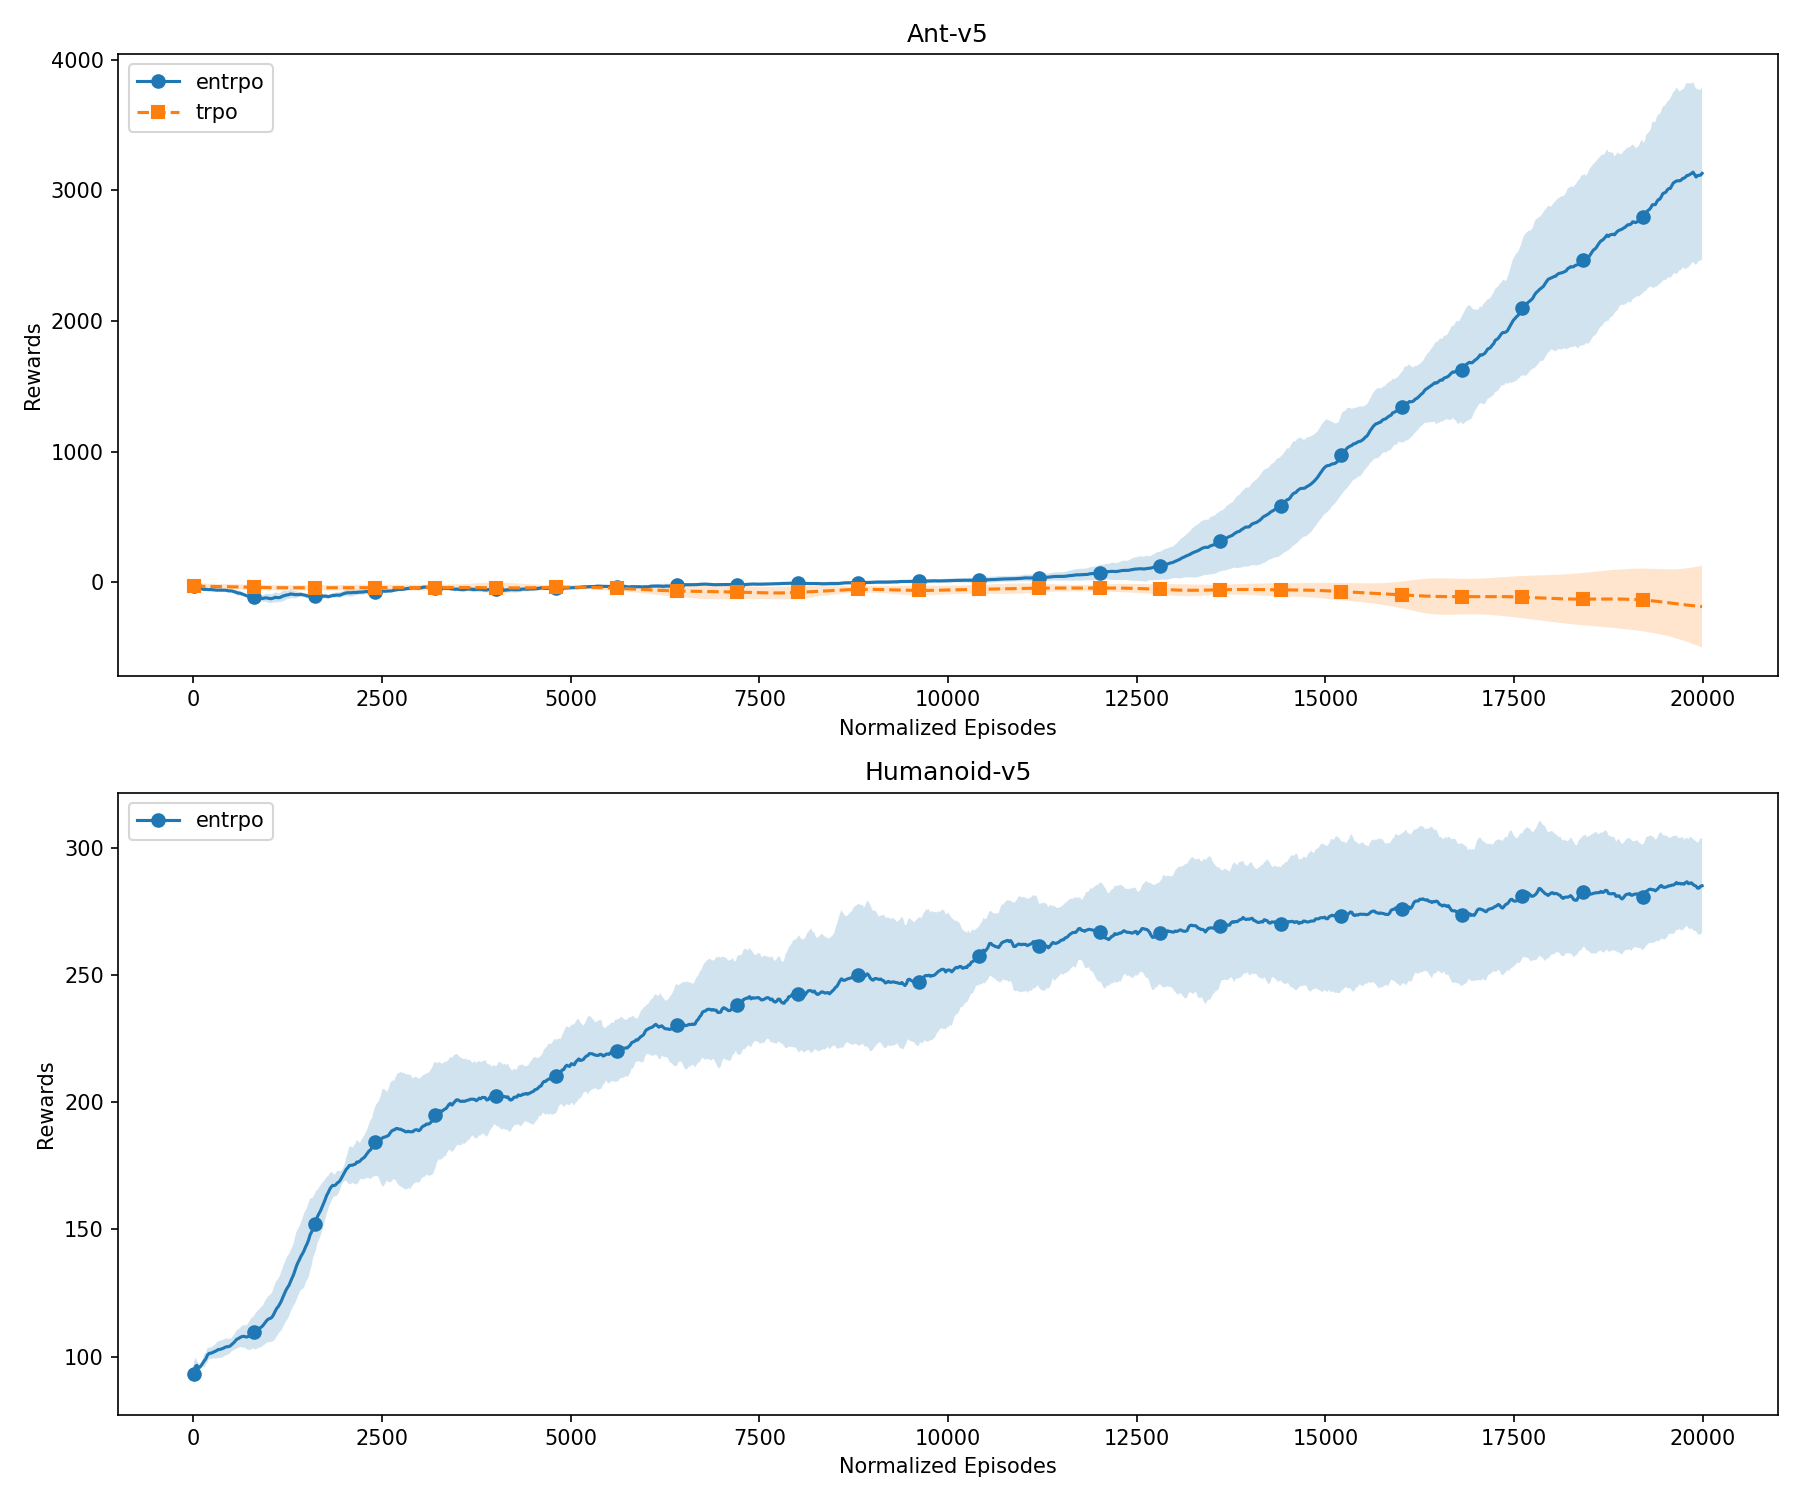
\includegraphics[width=0.8\textwidth]{.assets/resampled_outlier.png}
    \caption{Resampled Rewards with Outlier Removal}
\end{figure}

This plot presents reward distributions after applying smoothing and outlier removal techniques, filtering out misleading fluctuations.

\subsection*{Learning Stability}

\begin{figure}[H]
    \centering
    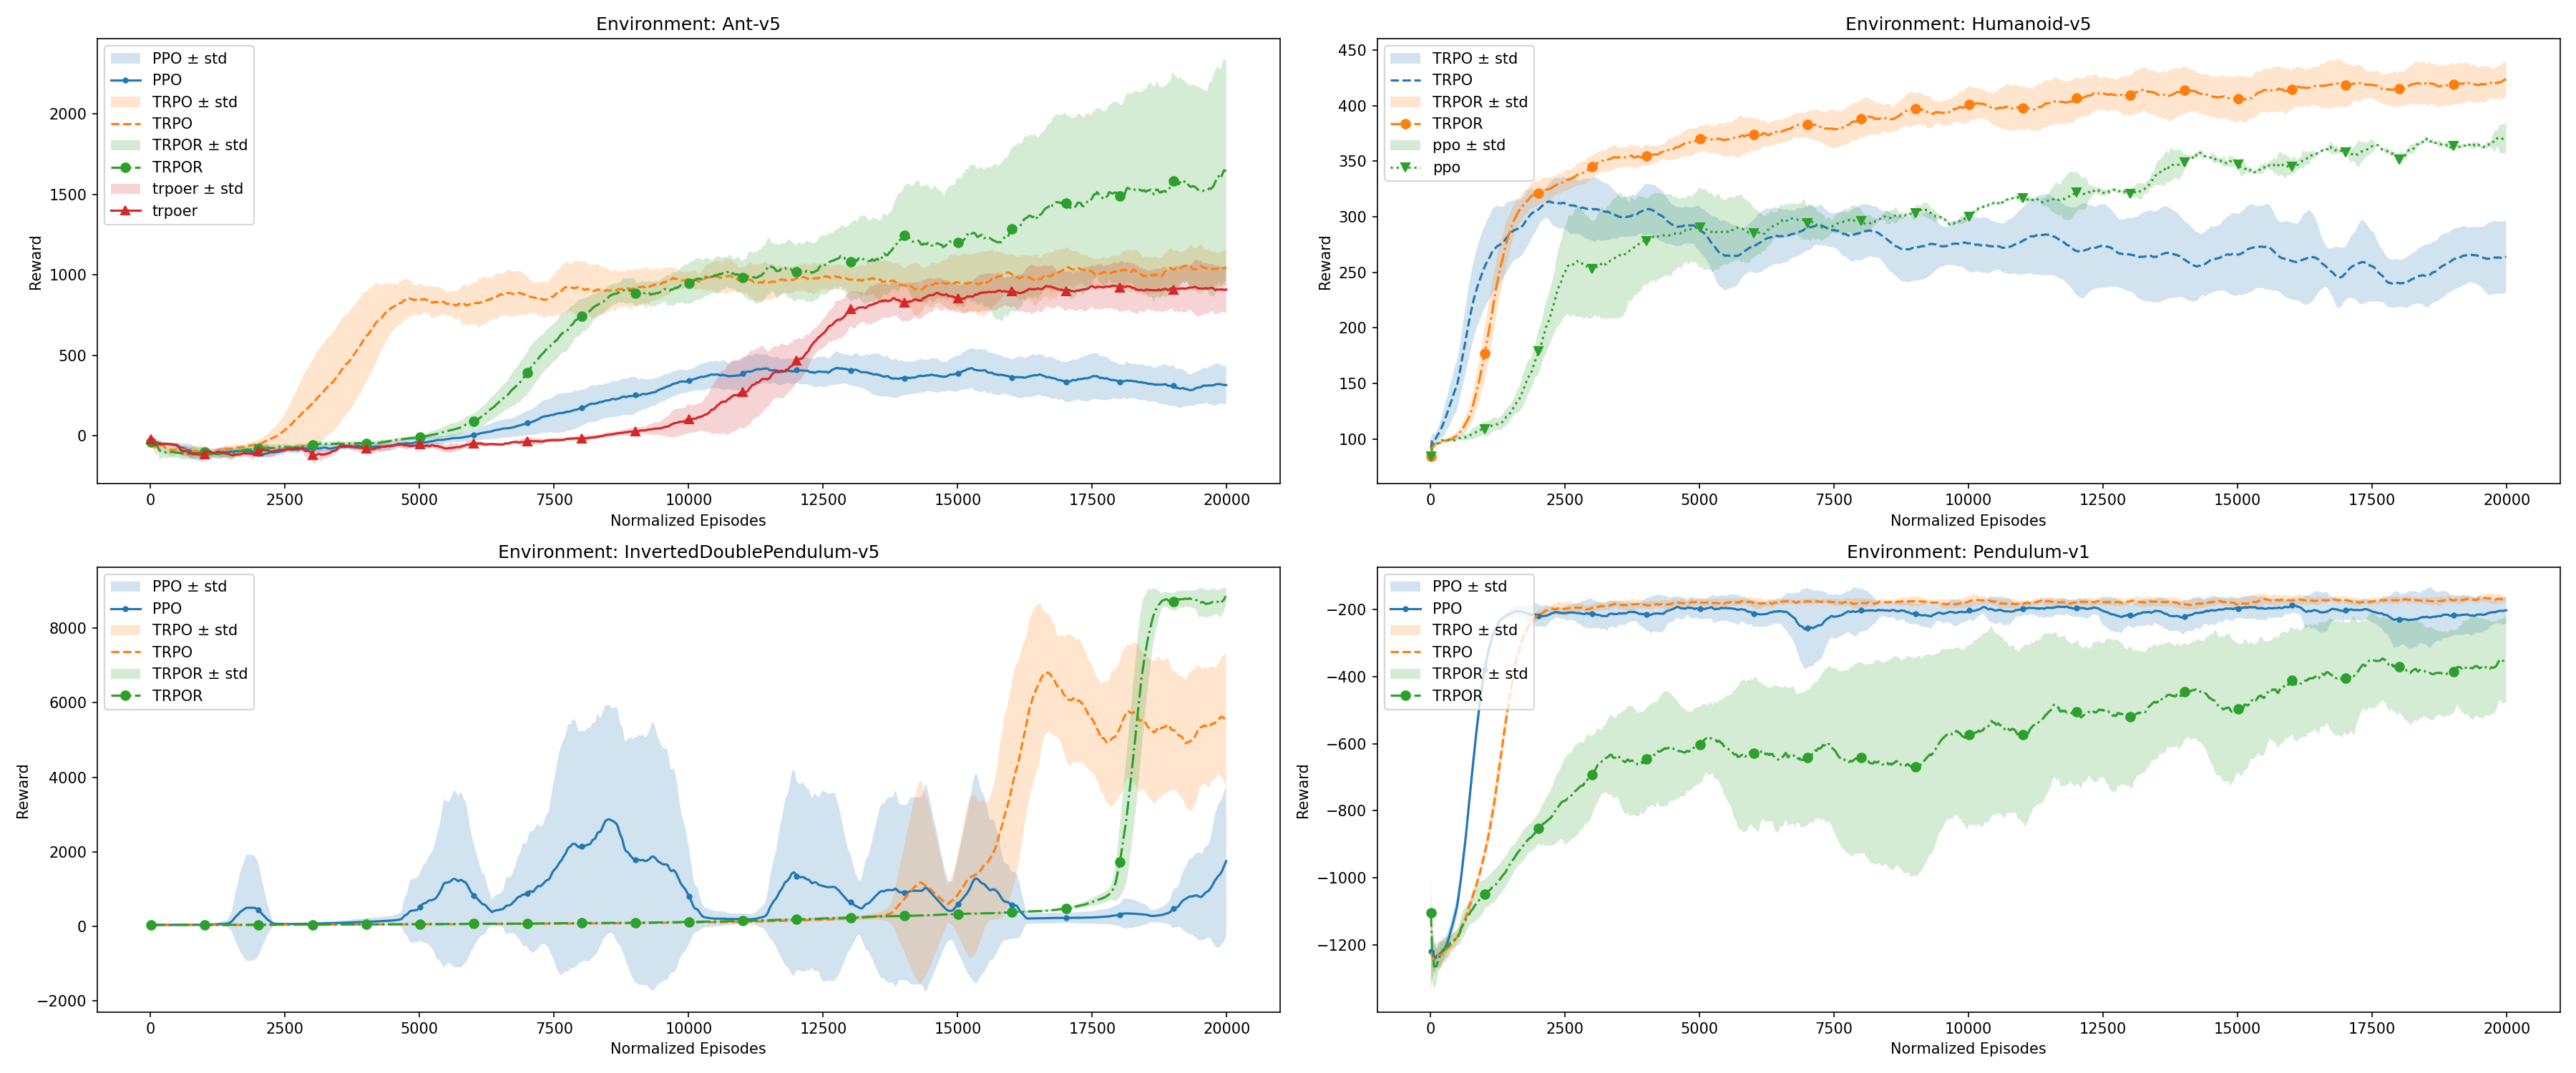
\includegraphics[width=0.8\textwidth]{.assets/learning_stability.png}
    \caption{Learning Stability for Different Models}
\end{figure}

Learning stability is evaluated based on the smoothness of the reward curve. A more stable learning process exhibits a steadily increasing reward trajectory, whereas high variance suggests instability due to sensitivity to hyperparameters.

\subsection*{Learning Stability (Coefficient of Variation)}

\begin{figure}[H]
    \centering
    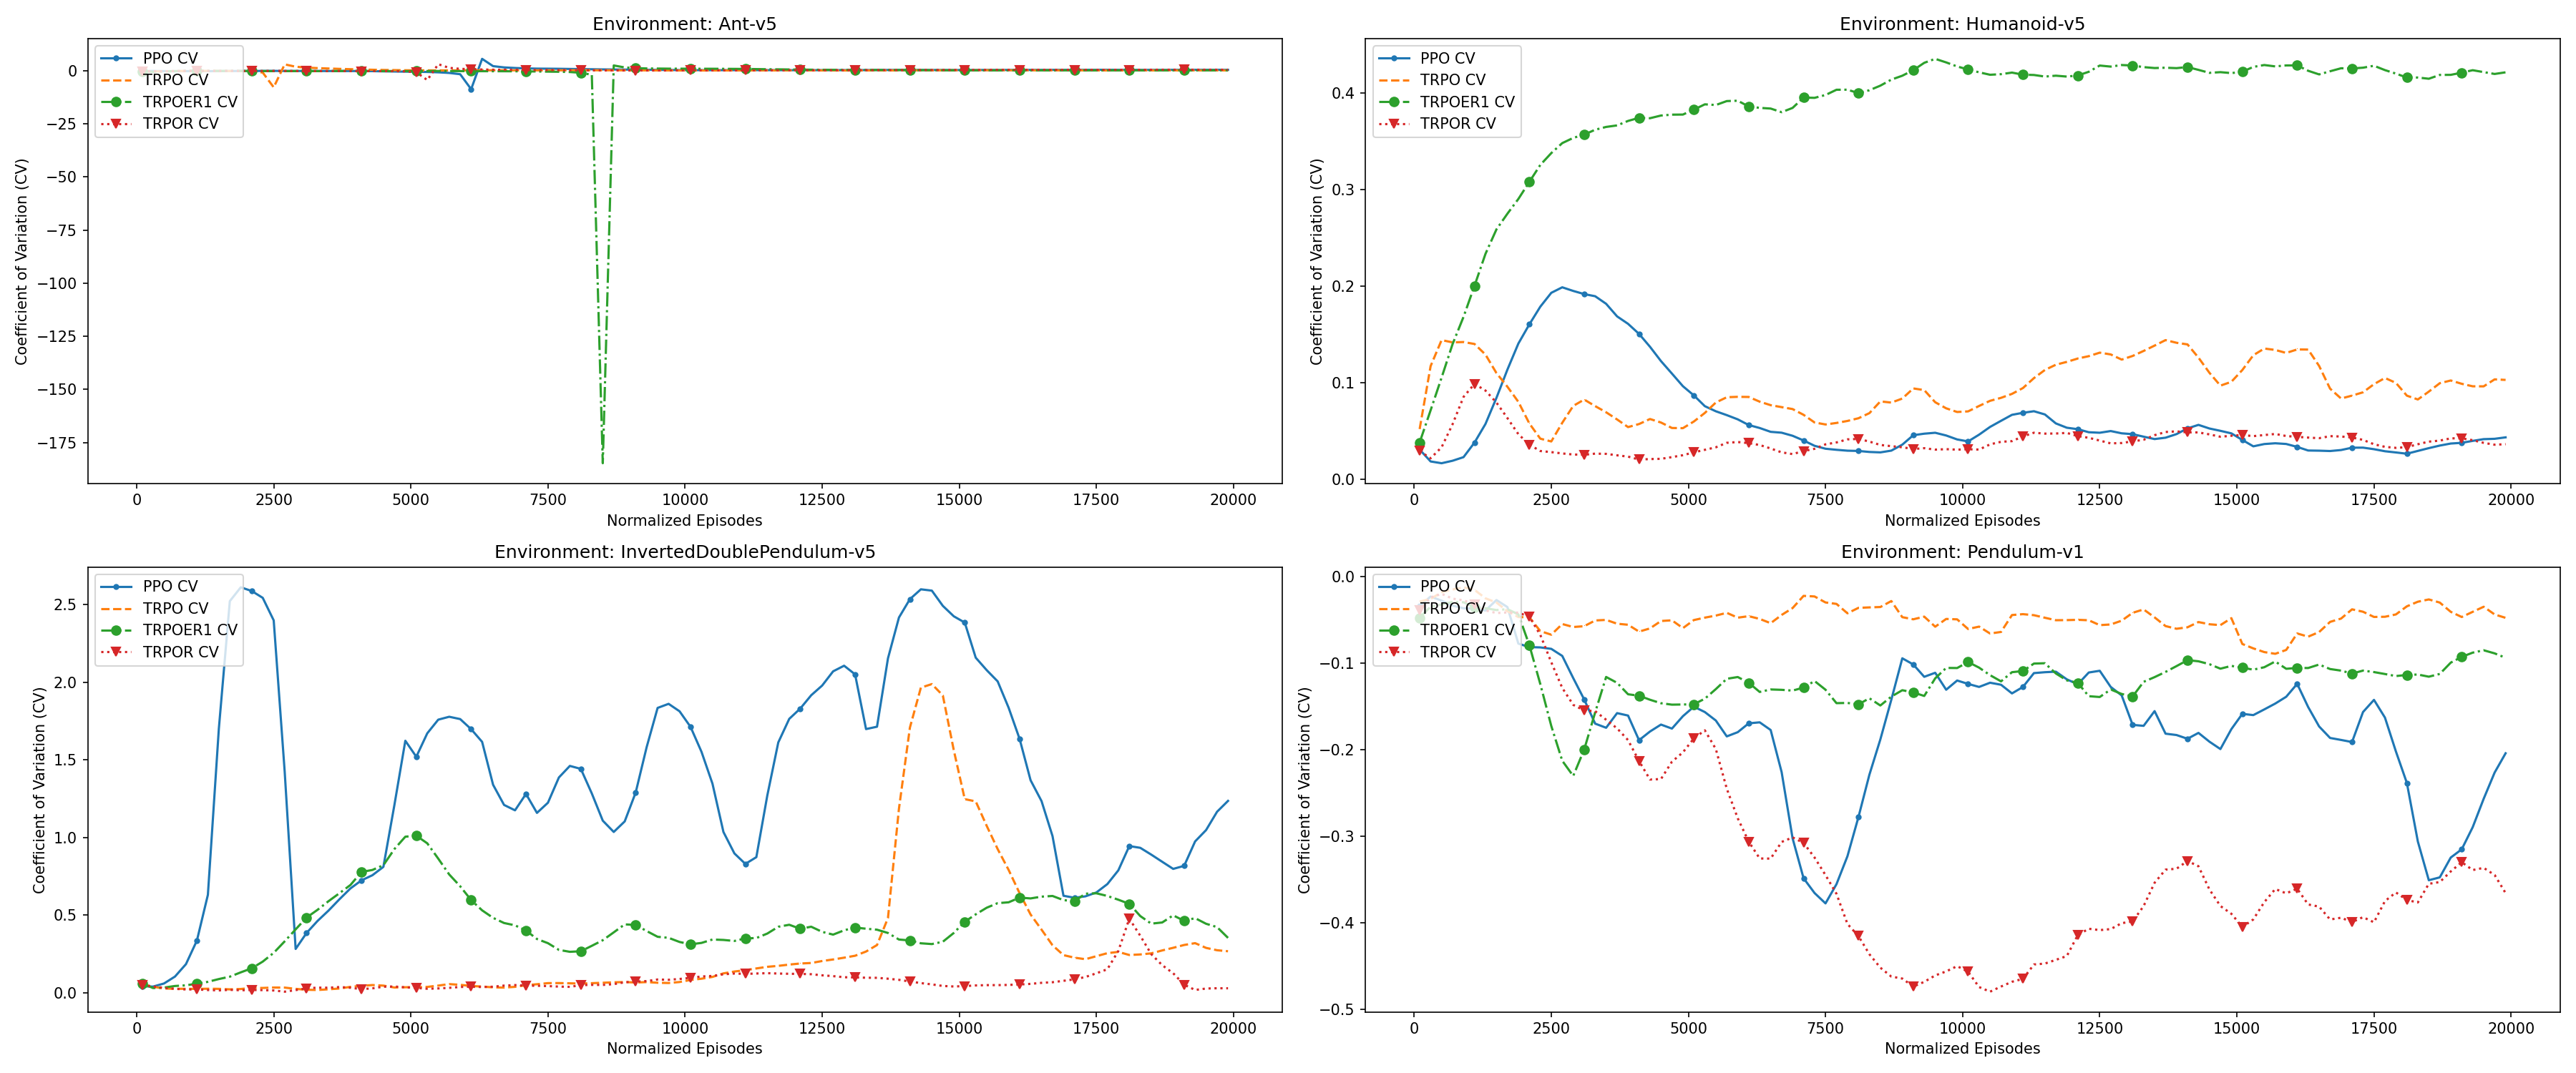
\includegraphics[width=0.8\textwidth]{.assets/learning_stability_cv.png}
    \caption{Learning Stability (Coefficient of Variation)}
\end{figure}

The coefficient of variation (CV) provides a normalized measure of stability. A lower CV signifies less volatile performance, whereas a higher CV indicates inconsistency due to randomness in training.

\subsection*{Sample Efficiency}

\begin{figure}[H]
    \centering
    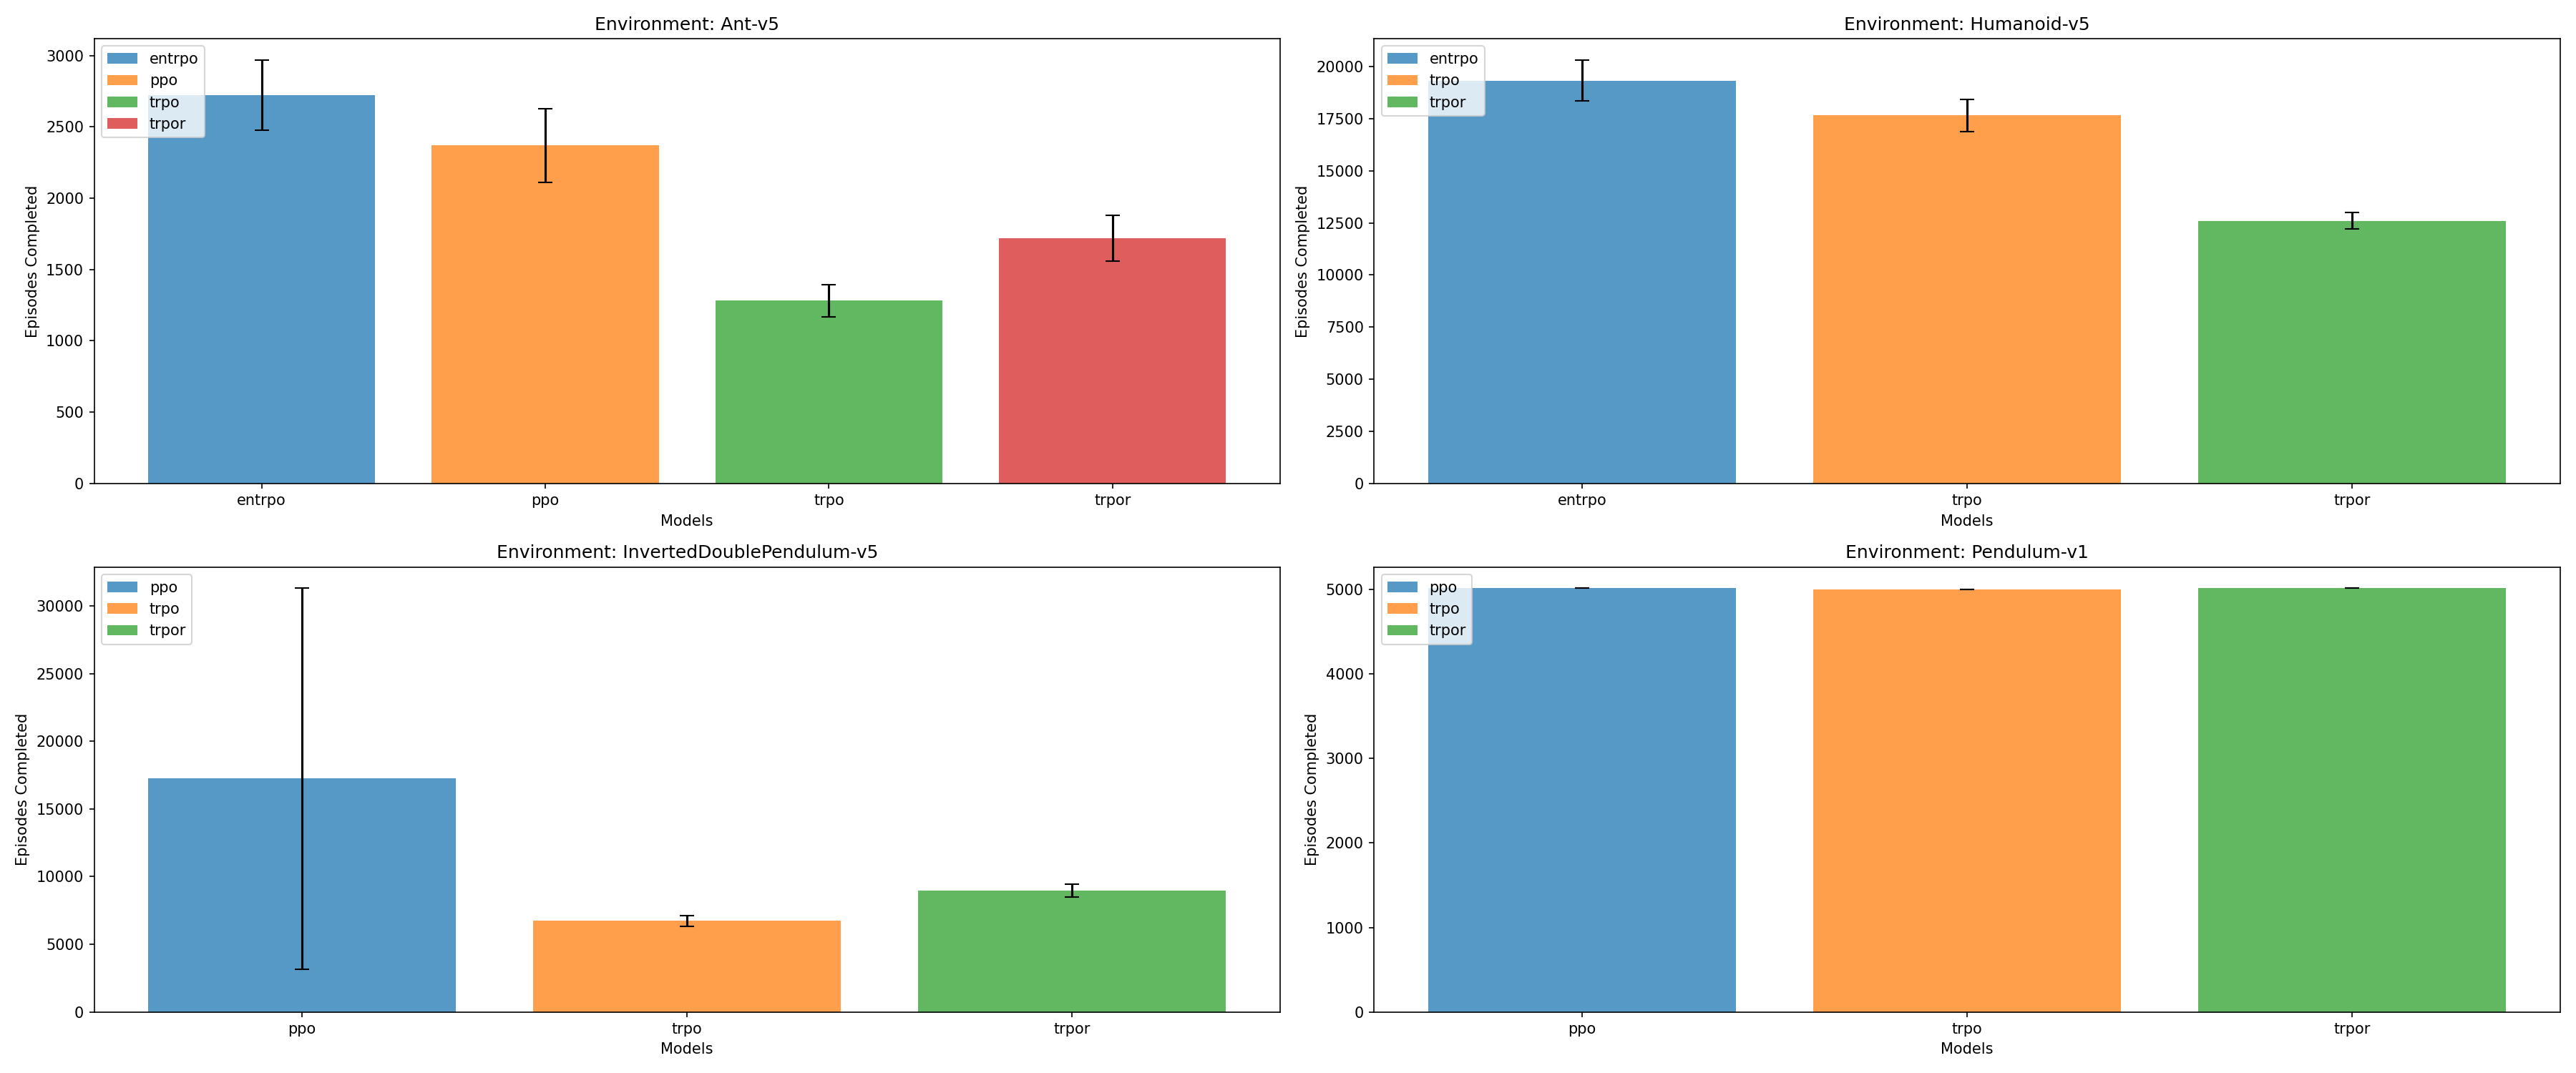
\includegraphics[width=0.8\textwidth]{.assets/sample_efficiency.png}
    \caption{Sample Efficiency Across Models}
\end{figure}

Sample efficiency measures how quickly a model improves with limited training episodes. Higher sample efficiency is desirable, especially in data-scarce scenarios.

\subsection*{Combined Sample Efficiency Results}

\begin{figure}[H]
    \centering
    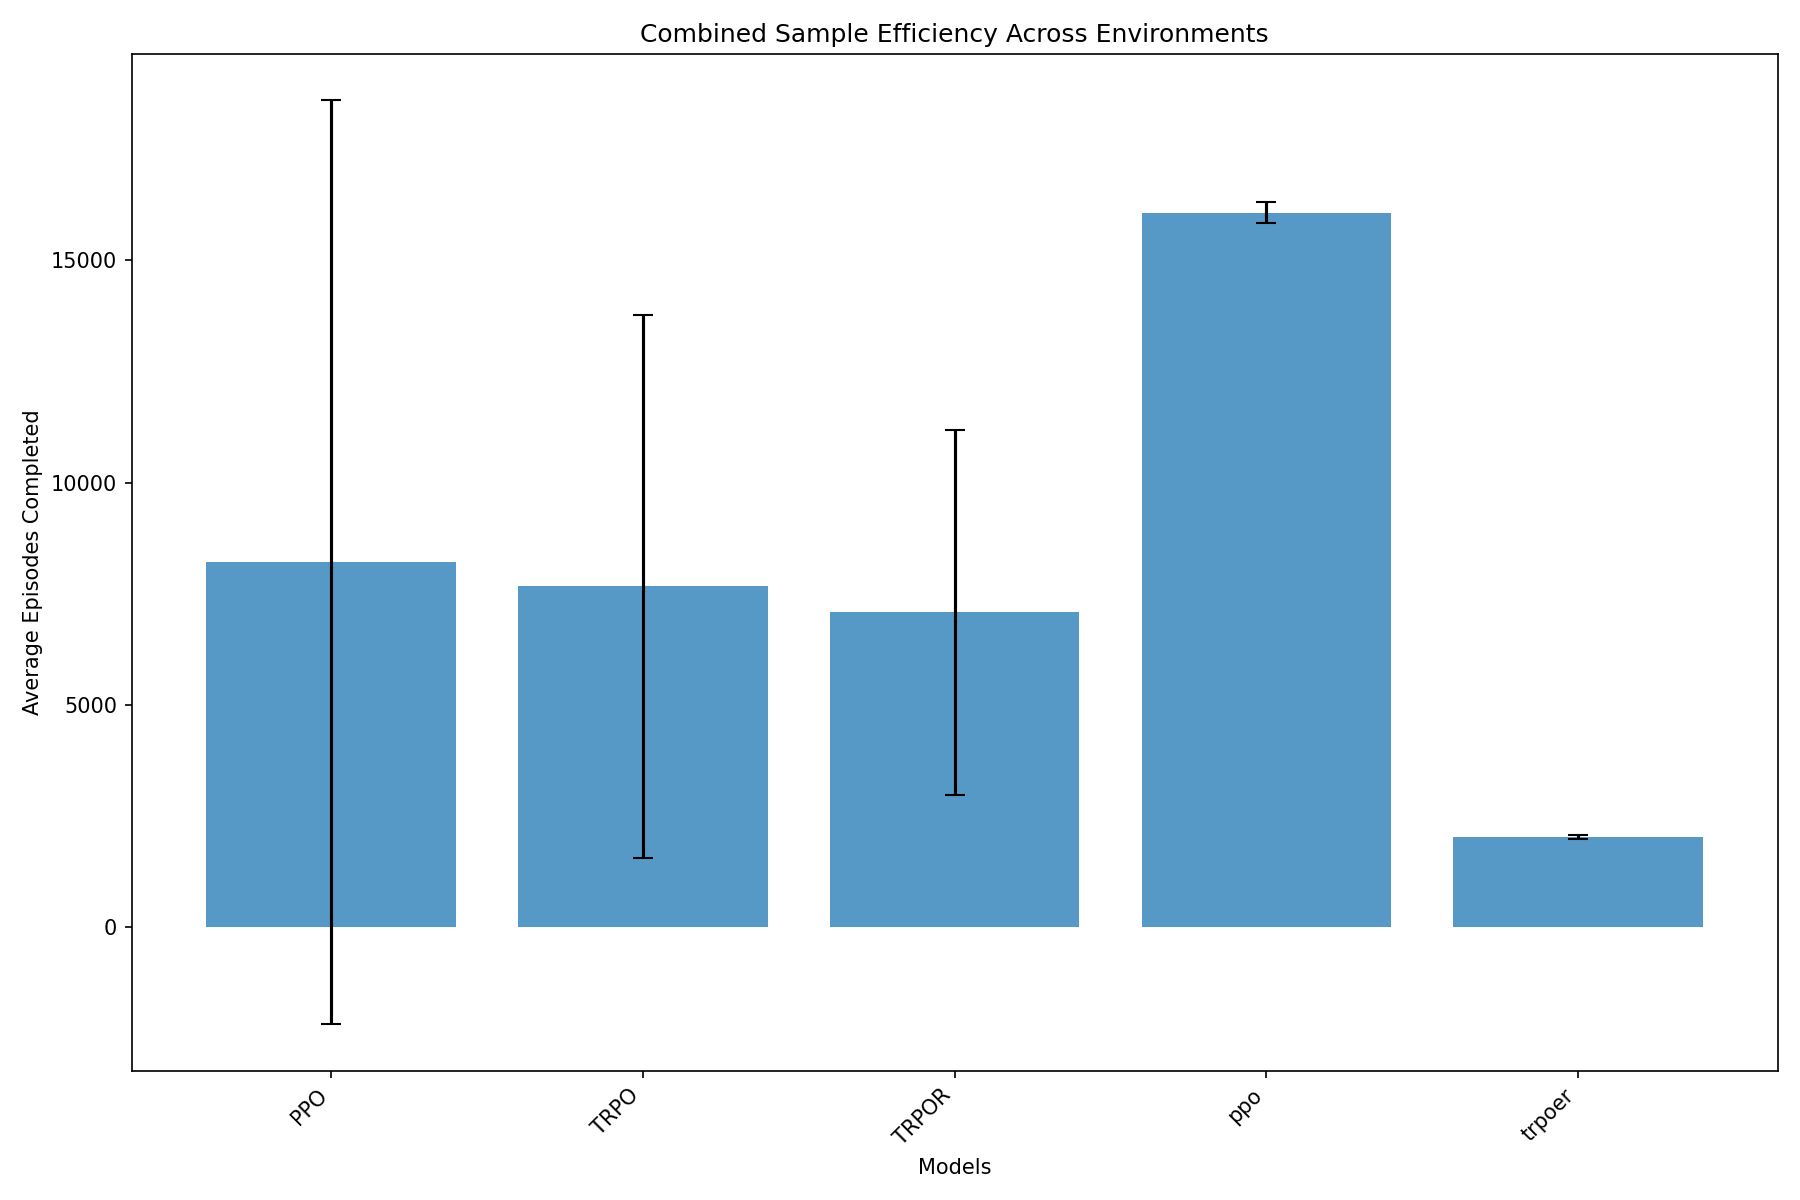
\includegraphics[width=0.8\textwidth]{.assets/sample_efficiency_combined.png}
    \caption{Combined Sample Efficiency Results}
\end{figure}

The combined sample efficiency plot aggregates results across all environments, showing how different models perform in terms of data efficiency.

\subsection*{Raw Data}

\begin{figure}[H]
    \centering
    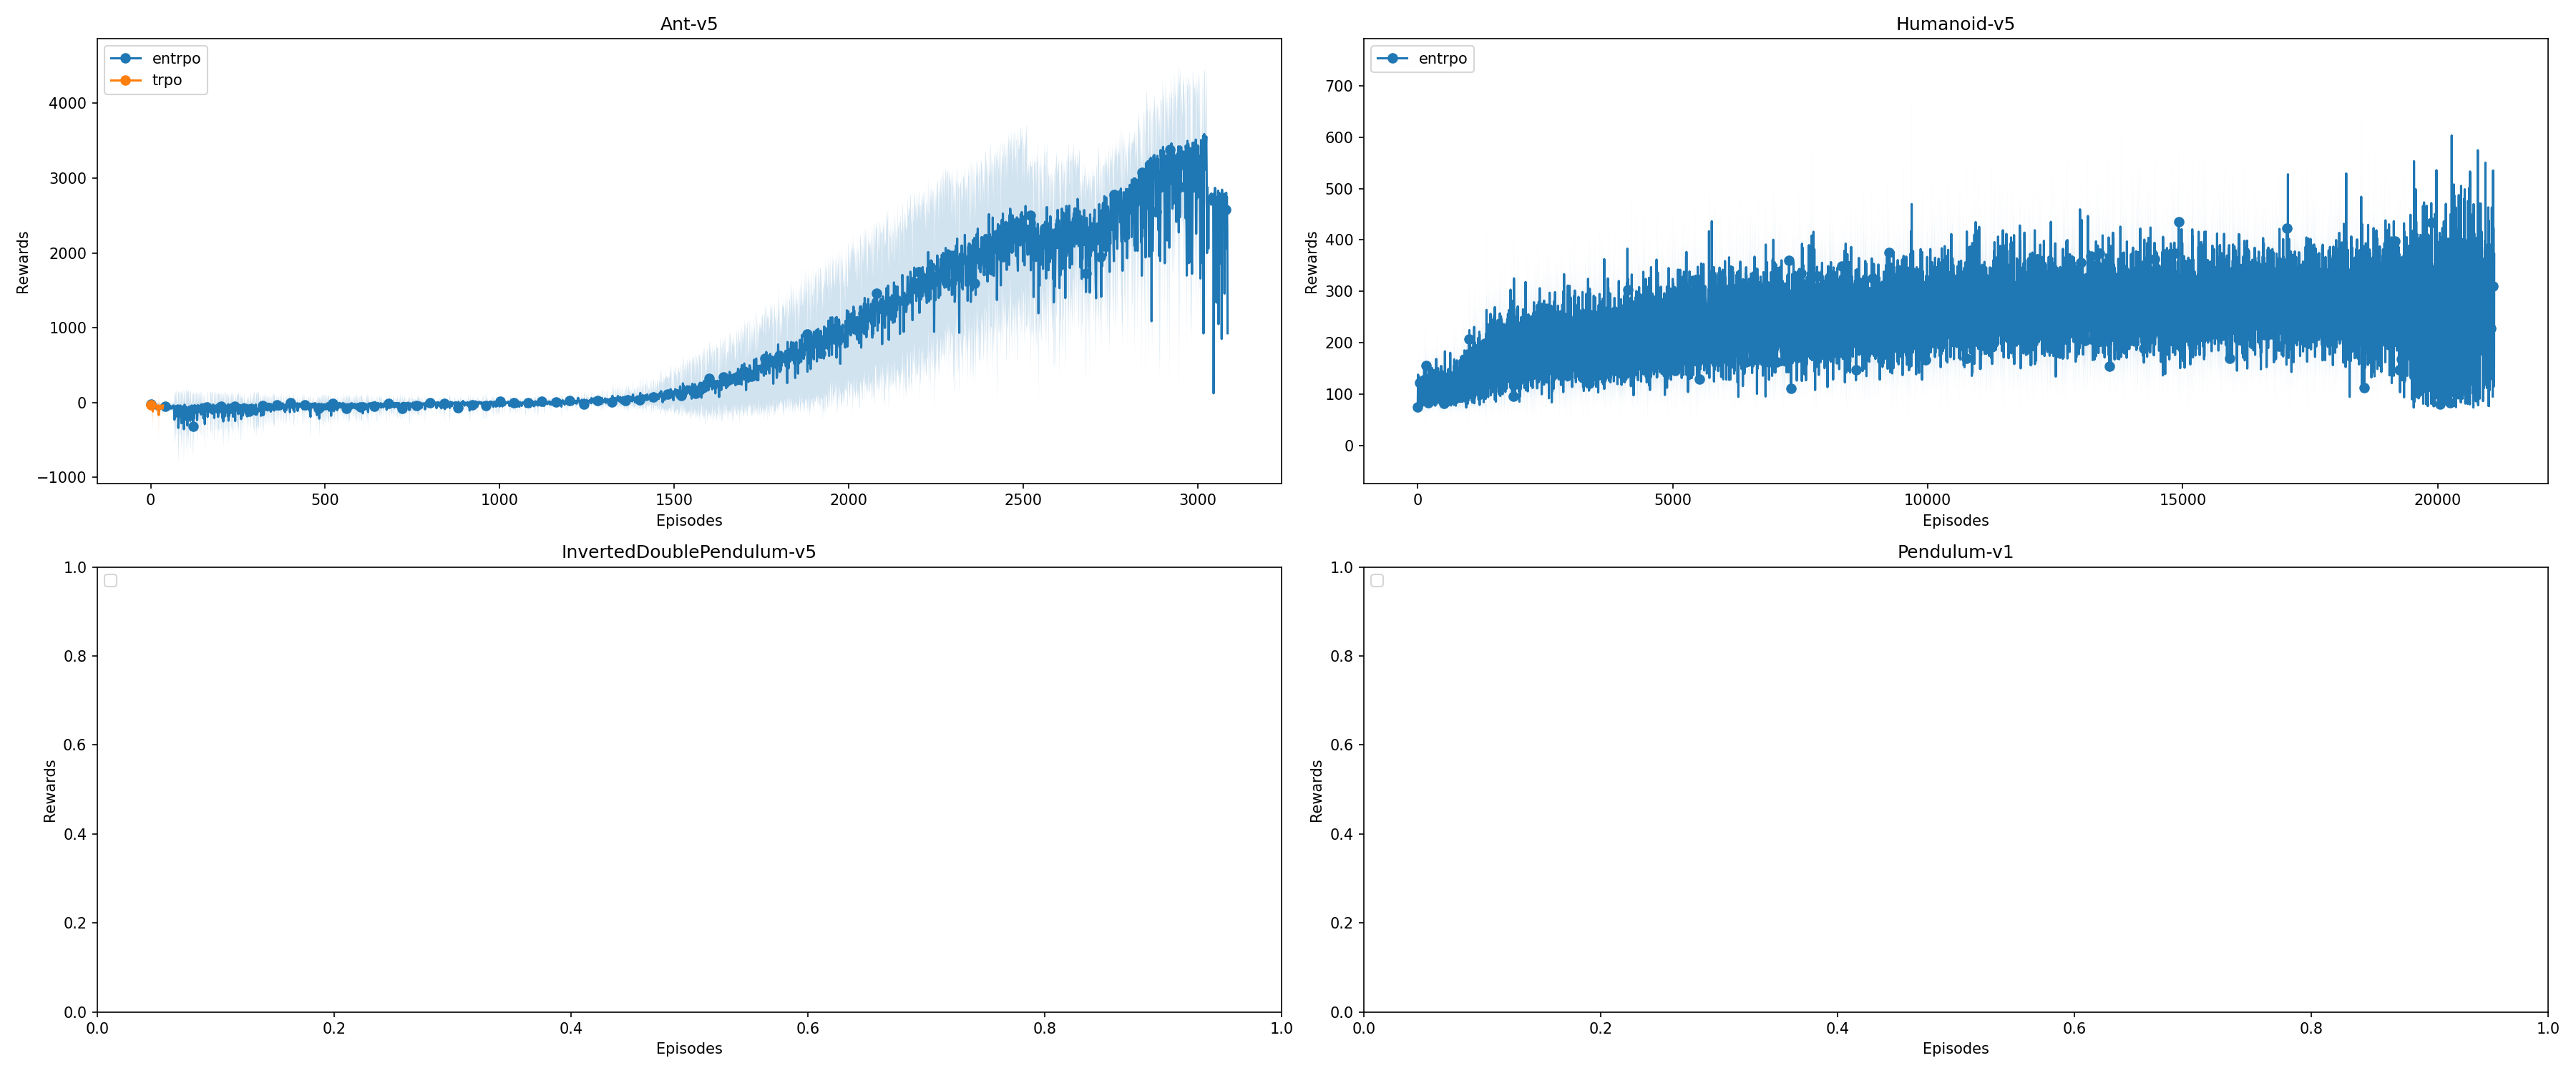
\includegraphics[width=0.8\textwidth]{.assets/raw_data.png}
    \caption{Raw Reward Data for Different Models}
\end{figure}

The raw data plot displays the recorded reward values without any smoothing. It provides insights into the actual training process and variability in rewards.

\newpage

\bibliographystyle{plain}
\bibliography{references}

\end{document}
